\section*{Problema 4} \label{sec:problema 4} 
Observem que en coordenades cartesianes, podem parametritzar la cardioide que té per equació \( r = 1 + \cos{\varphi} \) com
\begin{equation}
  \begin{aligned}
    x(\varphi) &= (1 + \cos{\varphi})\cos{\varphi} \\
    y(\varphi) &= (1 + \cos{\varphi})\sin{\varphi}
  \end{aligned}
	\label{eq:parametrització cardioide de revolució}
\end{equation}

amb \( \varphi \in (0, 2\pi) \). Per a parametritzar la superfície \( S \) que resulta quan la cardioide gira al voltant de l'eix \( x \) introduïm un nou paràmetre \( \theta \), que representarà l'angle de rotació. Com que la cardioide és simètrica, només ens cal la secció que correspon a \( \varphi \in (0, \pi) \). Podem parametritzar \( S \) mitjançant una funció \( H\colon (0,\pi) \times (0,2\pi) \longrightarrow \R^3 \) amb 
\begin{equation}
  H(\varphi,\theta) = ((1+\cos{\varphi})\cos{\varphi}, (1+\cos{\varphi})\sin{\varphi}\cos{\theta}, (1+\cos{\varphi})\sin{\varphi}\sin{\theta}). \label{eq:cardioide de revolució}
\end{equation}
És clar que \( H \) és un difeomorfisme en la seva imatge, i per tant defineix \( S \) com una varietat regular. Per ser rigurosos, amb aquesta parametrització ens deixem tot un arc del cardioide, que són tots els punts amb \( \theta = 0 \). Ara bé, a l'hora d'integrar no cal que ens preocupem ja que aquest conjunt té àrea nul·la. Si prenem com a domini de la parametrització \( [0,\pi] \times [0,2\pi] \)	obtenim tota la superfície.

\begin{figure}[htb]
  \centering
  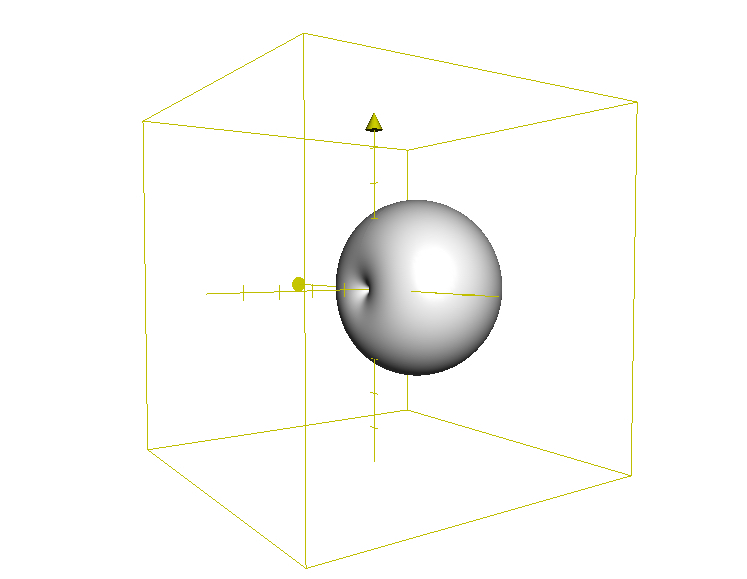
\includegraphics[scale = 0.4]{cardioide.jpg}
 	\caption{Resultat de la parametrització donada per \ref{eq:parametrització cardioide de revolució}} 
\end{figure}

Per calcular l'àrea d'una superfície donada per una parametrització hem de trobar l'element d'àrea i integrar-lo en el domini de la parametrització. Ara bé, podem aprofitar que \( S \) no és una varietat qualsevol, sino que és una superfície de revolució. En general, l'element d'àrea de la superfície de revolució que resulta de rotar l'arc \( \gamma(\varphi) = (x(\varphi), y(\varphi), 0) \) al voltant de l'eix \( x \) és 
\begin{equation}
  dA = y(\varphi)\norm{\dot{\gamma}(\varphi)} d\varphi \, d\theta = y(\varphi)\sqrt{\dot{x}(\varphi)^2 + \dot{y}(\varphi)^2} d\varphi \, d\theta. 
\end{equation}
A més, l'arc \( \gamma \) està donat en coordenades polars, així que és de la forma \( \gamma(\varphi) = r(\varphi) (\cos{\varphi}, \sin{\varphi}, 0) \) i per tant \( \norm{\dot{\gamma}(\varphi)} = \sqrt{r(\varphi)^2 + \dot{r}(\varphi)^2} \). Així doncs, l'àrea de \( S \), és a dir la mesura 2-dimensional de \( S \) és
\begin{align*}
 	m_2(S) &= \int_0^{2\pi} \! \int_0^\pi (1+\cos{\varphi})\sin{\varphi} \sqrt{(1+\cos{\varphi})^2 + \sin{\varphi}^2} \, d\varphi \, d\theta \\	
				 &= \int_0^{2\pi} \! \int_0^\pi (1+\cos{\varphi})\sin{\varphi} \sqrt{2(1 + \cos{\varphi})} \, d\varphi \, d\theta \\
				 &= -2\pi\sqrt{2} \int_0^\pi (1 + \cos{\varphi})^{3/2} \sin{\varphi} \, d\varphi \\ 
				 &= \left[-\dfrac{4\pi\sqrt{2}}{5} (1 + \cos{\varphi})^{5/2}\right]_0^\pi = \dfrac{32\pi}{5} 
\end{align*}

Observem que el punt \( \left(\frac{1}{2}(1+\sqrt{2}),\frac{1}{2}(1+\sqrt{2})\right) \) és precisament la imatge de \( \varphi = \pi/4 \) al cardioide. Així doncs, l'òrbita d'aquest punt quan fem girar el cardioide per generar \( S \) és el conjunt de punts de la forma \( H(\pi/4, \theta) \) amb \( \theta \in [0, 2\pi] \). Si volem calcular el pla tangent a \( S \) en qualsevol d'aquests punts, cal que avaluem les derivades parcials de \( H \) en aquests punts. Tenim
\begin{equation}
	\dfrac{\partial}{\partial \varphi}(\theta,\varphi) = \partial_{\varphi}H(\varphi, \theta) = \begin{bmatrix}
    -\sin{\varphi}(1 + 2\cos{\varphi}) \\
    (\cos{\varphi} + \cos{\varphi}^2 - \sin{\varphi}^2)\sin{\theta} \\
    (\cos{\varphi} + \cos{\varphi}^2 - \sin{\varphi}^2)\cos{\theta} 
  \end{bmatrix} \label{eq:parcial 1}
\end{equation}
i
\begin{equation}
	\dfrac{\partial}{\partial \theta}(\varphi, \theta) = \partial_{\theta}H(\varphi, \theta) = (1 + \cos{\varphi}) \begin{bmatrix}
    0 \\
    \sin{\varphi}\cos{\theta} \\
    -\sin{\varphi}\sin{\theta}
  \end{bmatrix} . \label{eq:parcial 2}
\end{equation}

El pla tangent a una superfície regular donada per una parametrització està generat per les derivades parcials de la parametrització. En els punts de l'òrbita que estem considerant ---és a dir, els punts amb \( \varphi = \pi/4 \)--- el pla tangent en funció de l'angle \( \theta \), \( \pi(\theta) \), està donat, com a subvarietat afí per
\begin{align*}
  \pi(\theta) &= H(\pi/4, \theta) + \left\langle \dfrac{\partial}{\partial \varphi}(\pi/4, \theta), \dfrac{\partial}{\partial \theta}(\pi/4, \theta) \right\rangle \\ 
							&= \dfrac{1+\sqrt{2}}{2} (1, \sin{\theta}, \cos{\theta}) \\
							& \quad +{} \left\langle \left(-\left(1+\sqrt{2}\right), \sin{\theta}, \cos{\theta}\right), (0, \cos{\theta}, -\sin{\theta}) \right\rangle \yestag \label{eq:multiplicar per escalars} .
\end{align*}
Al pas \ref{eq:multiplicar per escalars} s'ha dividit la parcial respecte de \( \theta \) per \( \frac{1}{\sqrt{2}}(1 + \sqrt{2}) \) i la parcial respecte de \( \varphi \) s'ha multiplicat per \( \sqrt{2} \). Fer això no afecta l'àlgebra lineal i alleugereix la notació.

Si volem donar una equació pel pla, observem que el vector \[ u = \left(1, \left(1+\sqrt{2}\right)\sin{\theta},  \left(1+\sqrt{2}\right)\cos{\theta}\right) \] és de l'ortogonal de \( \pi(\theta) \). Per tant, l'equació del pla tangent és:
\begin{equation*}
	\inn{u}{(x,y,z) - H(\pi/4, \theta)}.
\end{equation*}
Més en detall:
\begin{equation}
	x +\left(\left(1 + \sqrt{2}\right)\sin{\theta}\right)\! y +\left(\left(1 + \sqrt{2}\right)\cos{\theta}\right)\! z = \dfrac{4 + 3\sqrt{2}}{2}. 
\end{equation}



